% Options for packages loaded elsewhere
\PassOptionsToPackage{unicode}{hyperref}
\PassOptionsToPackage{hyphens}{url}
\PassOptionsToPackage{dvipsnames,svgnames,x11names}{xcolor}
%
\documentclass[
  12pt]{article}

\usepackage{amsmath,amssymb}
\usepackage{iftex}
\ifPDFTeX
  \usepackage[T1]{fontenc}
  \usepackage[utf8]{inputenc}
  \usepackage{textcomp} % provide euro and other symbols
\else % if luatex or xetex
  \usepackage{unicode-math}
  \defaultfontfeatures{Scale=MatchLowercase}
  \defaultfontfeatures[\rmfamily]{Ligatures=TeX,Scale=1}
\fi
\usepackage{lmodern}
\ifPDFTeX\else  
    % xetex/luatex font selection
\fi
% Use upquote if available, for straight quotes in verbatim environments
\IfFileExists{upquote.sty}{\usepackage{upquote}}{}
\IfFileExists{microtype.sty}{% use microtype if available
  \usepackage[]{microtype}
  \UseMicrotypeSet[protrusion]{basicmath} % disable protrusion for tt fonts
}{}
\makeatletter
\@ifundefined{KOMAClassName}{% if non-KOMA class
  \IfFileExists{parskip.sty}{%
    \usepackage{parskip}
  }{% else
    \setlength{\parindent}{0pt}
    \setlength{\parskip}{6pt plus 2pt minus 1pt}}
}{% if KOMA class
  \KOMAoptions{parskip=half}}
\makeatother
\usepackage{xcolor}
\setlength{\emergencystretch}{3em} % prevent overfull lines
\setcounter{secnumdepth}{5}
% Make \paragraph and \subparagraph free-standing
\ifx\paragraph\undefined\else
  \let\oldparagraph\paragraph
  \renewcommand{\paragraph}[1]{\oldparagraph{#1}\mbox{}}
\fi
\ifx\subparagraph\undefined\else
  \let\oldsubparagraph\subparagraph
  \renewcommand{\subparagraph}[1]{\oldsubparagraph{#1}\mbox{}}
\fi


\providecommand{\tightlist}{%
  \setlength{\itemsep}{0pt}\setlength{\parskip}{0pt}}\usepackage{longtable,booktabs,array}
\usepackage{calc} % for calculating minipage widths
% Correct order of tables after \paragraph or \subparagraph
\usepackage{etoolbox}
\makeatletter
\patchcmd\longtable{\par}{\if@noskipsec\mbox{}\fi\par}{}{}
\makeatother
% Allow footnotes in longtable head/foot
\IfFileExists{footnotehyper.sty}{\usepackage{footnotehyper}}{\usepackage{footnote}}
\makesavenoteenv{longtable}
\usepackage{graphicx}
\makeatletter
\def\maxwidth{\ifdim\Gin@nat@width>\linewidth\linewidth\else\Gin@nat@width\fi}
\def\maxheight{\ifdim\Gin@nat@height>\textheight\textheight\else\Gin@nat@height\fi}
\makeatother
% Scale images if necessary, so that they will not overflow the page
% margins by default, and it is still possible to overwrite the defaults
% using explicit options in \includegraphics[width, height, ...]{}
\setkeys{Gin}{width=\maxwidth,height=\maxheight,keepaspectratio}
% Set default figure placement to htbp
\makeatletter
\def\fps@figure{htbp}
\makeatother

\addtolength{\oddsidemargin}{-.5in}%
\addtolength{\evensidemargin}{-1in}%
\addtolength{\textwidth}{1in}%
\addtolength{\textheight}{1.7in}%
\addtolength{\topmargin}{-1in}%
\makeatletter
\@ifpackageloaded{caption}{}{\usepackage{caption}}
\AtBeginDocument{%
\ifdefined\contentsname
  \renewcommand*\contentsname{Table of contents}
\else
  \newcommand\contentsname{Table of contents}
\fi
\ifdefined\listfigurename
  \renewcommand*\listfigurename{List of Figures}
\else
  \newcommand\listfigurename{List of Figures}
\fi
\ifdefined\listtablename
  \renewcommand*\listtablename{List of Tables}
\else
  \newcommand\listtablename{List of Tables}
\fi
\ifdefined\figurename
  \renewcommand*\figurename{Figure}
\else
  \newcommand\figurename{Figure}
\fi
\ifdefined\tablename
  \renewcommand*\tablename{Table}
\else
  \newcommand\tablename{Table}
\fi
}
\@ifpackageloaded{float}{}{\usepackage{float}}
\floatstyle{ruled}
\@ifundefined{c@chapter}{\newfloat{codelisting}{h}{lop}}{\newfloat{codelisting}{h}{lop}[chapter]}
\floatname{codelisting}{Listing}
\newcommand*\listoflistings{\listof{codelisting}{List of Listings}}
\makeatother
\makeatletter
\makeatother
\makeatletter
\@ifpackageloaded{caption}{}{\usepackage{caption}}
\@ifpackageloaded{subcaption}{}{\usepackage{subcaption}}
\makeatother
\ifLuaTeX
  \usepackage{selnolig}  % disable illegal ligatures
\fi
\usepackage[]{natbib}
\bibliographystyle{agsm}
\usepackage{bookmark}

\IfFileExists{xurl.sty}{\usepackage{xurl}}{} % add URL line breaks if available
\urlstyle{same} % disable monospaced font for URLs
\hypersetup{
  pdftitle={Estimating ``Contact Zones'' for NFL Defenders to Improve Tackling Tracking},
  pdfauthor={Dennison Jackson},
  pdfkeywords={American football, tackling, defense analysis, tracking
data},
  colorlinks=true,
  linkcolor={blue},
  filecolor={Maroon},
  citecolor={Blue},
  urlcolor={Blue},
  pdfcreator={LaTeX via pandoc}}


\begin{document}


\def\spacingset#1{\renewcommand{\baselinestretch}%
{#1}\small\normalsize} \spacingset{1}


%%%%%%%%%%%%%%%%%%%%%%%%%%%%%%%%%%%%%%%%%%%%%%%%%%%%%%%%%%%%%%%%%%%%%%%%%%%%%%

\date{May 10, 2024}
\title{\bf Estimating ``Contact Zones'' for NFL Defenders to Improve
Tackling Tracking}
\author{
Dennison Jackson\\
Department of Statistics, Kansas State University\\
}
\maketitle

\bigskip
\bigskip
\begin{abstract}
This paper introduces a method for estimating ``contact zones'' around
defenders in American football using NFL Next Gen Stats, with the goal
of opening up the field for future research into tackling. Currently,
there is not much research being done on tackling using player data.
Part of the issue is that it can be difficult to discern when a tackle
begins in the data, especially in cases where there are multiple
tacklers on a play. We focus on establishing zones around defenders such
that if a ball-carrier enters a defender's zone, it is reasonable to
assume that contact has initiated. We develop several metrics with the
goal of figuring out an optimal radius for our zones that aligns with
real-world tackle events. Our findings suggest that a zone with a radius
of 1.2 yards around defenders offers a reliable estimate for initiating
contact. The implemetation of these zones will help advance future
research by allowing for better analysis of individual tackles as well
as the ability to analyze multiple tacklers on the same play.
\end{abstract}

\noindent%
{\it Keywords:} American football, tackling, defense analysis, tracking
data
\vfill

\newpage
\spacingset{1.9} % DON'T change the spacing!

\section{Introduction}\label{introduction}

For the past six years, the National Football League (NFL) has hosted a
``Big Data Bowl'' contest on the data science competition platform
Kaggle \citep{BDB, Kaggle}. Each competition has its own theme that
revolves around some aspect of American football; in 2024, this theme
was tackling. Contestants were asked to come up with new metrics or
coaching strategies revolving around tackling by analyzing the NFL's
Next Gen Stats \citep{NextGenStats}. This data consists of player
tracking data, which includes coordinates of every player along with
their orientation, speed, and acceleration among numerous other
statistics which are collected at a frequency of ten frames a second for
every play in every game. The NFL published Next Gen Stats for plays
involving tackles for the first nine weeks for the 2022-2023 season onto
Kaggle, along with supplementary datasets that include detailed
information about individual plays, games, players, and tackles.

The end goal of the project is open-ended, but one of the main tracks
involved the creation of metrics based around tackling. Originally, the
goal of this paper was to follow this track and develop our own new
statistic, but along the way, we ran into a question that shifted our
perspective and led to a new project entirely: ``When does a tackle
start in the tracking data?'' Most metrics we were considering dealt
with analyzing what happens during a tackle, and in order to calculate
anything related to that we need to know roughly when a tackle begins
and ends.

When first glancing at the data, this may not be an obvious issue. In
the tracking data, there is a variable labeled event, which consists of
labels for significant events that happen during a play. Most of the
values are missing, but on certain frames you may see ``pass\_caught'',
``ball\_snap'', or ``fumble'' among others. Two of those others include
``tackle'' and ``first\_contact.'' A frame with an event of ``tackle''
provides a clear end to the tackle, as that is the moment the
ball-carrier was officially marked as being down, meaning the play is
over. ``first\_contact'' is a different story--it represents the first
moment in a play that any defender made contact with a ball-carrier.
This may seem like a good indicator of when a tackle starts, but there
are some major issues with using it as such.

First contact happening does not guarantee a tackle happened from that
contact. It is not unusual for a ball-carrier to be contacted by a
defender and a) break free of the tackle or b) be tackled shortly after
by a different defender. Both of these cases could cause serious issues
with our metrics if we treat first contact as the beginning of any
tackle. Even if we assumed that to be true, there is another glaring
issue: what happens when there are multiple tacklers on a play? A tackle
is not limited to one player, multiple tacklers can be credited as
having made one on the same play. The event ``first\_contact'' cannot
account for this, it only tells us when the first defender first made
contact, but nothing about any of the other defenders.

In this paper, we will be defining a new way to identify when a tackle
begins using the tracking data. We will do this by creating a ``contact
zone'' around certain defenders, such that if the ball-carrier is within
a defender's zone, it is reasonable to assume that the defender is
making contact with them. If we can estimate the size of the zone well,
we will be able to get an approximation of when any defender starts
making contact with the ball-carrier for any given play. This opens up
the door for future research if we are wanting to study anything across
the duration of a tackle or any case where we want to analyze the
tackling of multiple defenders on a play.

\subsection{Previous Work}\label{previous-work}

As NFL Next Gen Stats are relatively new, especially to the public,
there is not much research involving them. There's even less research
around its applications on the defensive side of the field; most papers
tend to focus on the offense. \citet{Yurko2020} explore using Next Gen
Stats to continuously model game outcomes such as the expected number of
yards a ball-carrier will make it on a play. While the focus of the
analysis is on the ball-carrier, they do derive measures relating to the
defenders, such as how close defenders are to the ball-carrier at every
point in the play. They also use Voronoi tessellations to divide the
entire field into zones, where each player has a region representing the
area on the field closest to them.

\citet{STRAIN} uses player tracking data create a new metric called
STRAIN that evaluates the effectiveness of a defense's pass rush on how
effectively they can break through the offensive line and put pressure
on the quarterback. This analysis does not involve tackling or contact,
but rather looks at the speeds of defenders and their distance to the
quarterback. \citet{Eager} also uses the Next Gen Stats to develop
metrics centered around linebackers, though these do not involve tacking
either.

While there has been extensive research done on tracking data from other
sports such as basketball or soccer/football, there are not many sports
with this data that are contact sports in the same way American football
is. \citet{Gudmundsson} has a great overview of applications of tracking
data in a wide variety of sports. \citet{wideopenspaces} uses football
(soccer) tracking data to analyze how players control and influence the
space around them.

Not much research has been done into defining zones for physical contact
around players. Motivated by the COVID-19 pandemic, \citet{covid} has a
paper that uses football (soccer) tracking data to identify contact
between players that potentially causes exposure to viruses. They
monitor the amount of time players and referees are within 2m of each
other with the goal of judging whether or not there is a risk of a
disease spreading.

\section{Methodology}\label{methodology}

In this paper, we choose to only estimate contact zones for all
defensive backs and linebackers, from here on referred to collectively
as defenders of interest (DOI). This includes all defenders except for
defensive linemen. One major factor for this decision has to do with
blockers. In any play, the offensive players that do not have the ball
are usually trying to block the defenders to stop them from reaching the
ball-carrier. While players of any position can be blocked, this tends
to happen more to defensive linemen then any other defender, as right
when the play starts, they immediately start grappling with the
offensive linemen. The idea of a contact zone assumes that there is
nothing impeding the defender from reaching the ball-carrier, so when a
ball-carrier runs through a gap in the line, it is highly likely they
will enter the contact zones for linemen, but the linemen will not be
able to reach them to do another player being in-between them. Since my
zones do not account for blockers, and defensive linemen tend to be
blocked the most, we excluded them from this analysis and have left that
for future work. Since linemen also have a different role to play than
other defenders (they are focused on sacking the quarterback and
preventing primarily runs as opposed to passes), their contact zone may
differ in size from the ones assigned to a DOI, and should potentially
be estimated separately.

\begin{figure}

\centering{

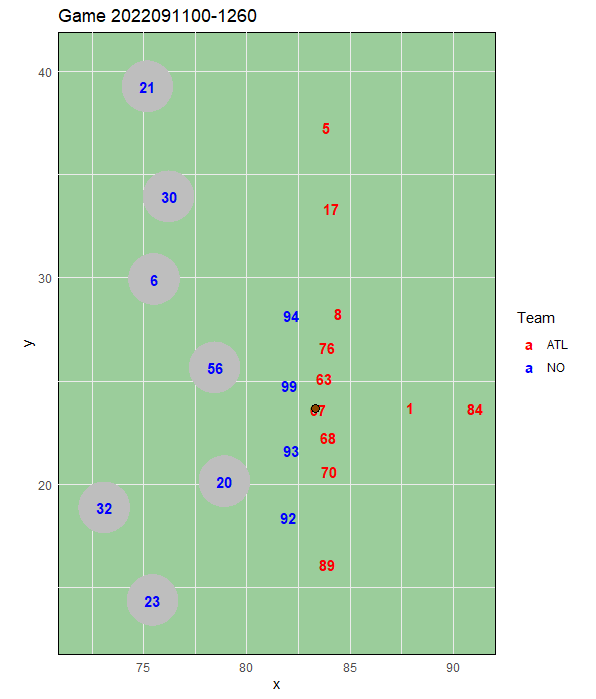
\includegraphics[width=3.125in,height=\textheight]{Images/ZoneExample.png}

}

\caption{\label{fig-zones}Example starting frame of a play with
theoretical contact zones show in gray around defenders of interest. The
ball is represented by a brown circle.}

\end{figure}%

\subsection{Data Preparation}\label{data-preparation}

For this analysis, we decided to only consider data from the first week
of the 2022-2023 NFL season, but everything done here is scalable and
could be easily applied to more seasons at the expensive of a higher
runtime. To prepare the data for analysis, we create four new variables:

\begin{itemize}
\item
  gamePlayId: a combination of the gameId and playId for a play in the
  form gameId-playId
\item
  doi\_ind: A dummy variable with a value of 1 is the player is a
  defender of interest, and 0 if not.
\item
  bc\_ind: A dummy variable with a value of 1 if the player is the
  ball-carrier, and 0 if not.
\item
  bcInZone: A dummy variable with a value of 1 if the distance from the
  ball-carrier to a defender of interest is less than the proposed
  radius of the contact zone, and a 0 if not.
\end{itemize}

We then filter the plays to only include those where a tackle was
performed by at least one defender of interest. Next, we extract the
ball-carrier's information from each play, namely their x and y
coordinates on the field. Then, we join these coordinates back with each
of the DOIs coordinates to calculate the Euclidean distance to the ball
carrier at every frame on a play.

We also apply a filter to the bcInZone indicator if the play involves a
pass. For any play with the events ``pass\_arrived'' or ``pass\_caught''
we set the value of bcInZone to 0 until the pass has arrived. We need to
do this because otherwise the ball-carrier is treated as an active
ball-carrier before they have even recieved the ball. This means that as
they are running their route, they may be passing through DOI's contact
zones, which can throw off our results and indicate that there were more
players active in the tackle than there actually were. It is illegal to
start tackling a player before they have the ball, so until then no
zones should be activated. Once they are in possession of the ball, they
are fair game to be tackled and thus the indicator is reactivated.

After this, the preliminary data filtering is done and we can start work
on evaluating the size of a contact zone.

\subsection{Evaluating a contact zone}\label{evaluating-a-contact-zone}

We define a contact zone as a circle with radius \(r\) centered around a
defender. We wish to figure out the optimal value for \(r\), such that
the size of the zone accurately approximates the start of a tackle. Say,
for instance, we decide on a radius of \(r = 1.5\) yards. This would
mean that whenever a ball-carrier is 1.5 yards away from a defender of
interest, we want to assume they are able to begin making contact at
approximately that point. In order to evaluate how good of an
approximation a zone with radius \(r\) is, we propose five metrics that
can potentially indicate if one radius is better than another.

Our first two metrics go hand-in-hand; we call them meanEntryDiff and
medianEntryDiff. These represent the average and median differences
between the frame the event ``first\_contact'' occurred on and the first
frame that the ball-carrier entered a contact zone on a play. So for
instance, if the difference between first contact and the first entry
into a contact zone is 10, that means our zone is saying contact started
10 frames (or one second) before the data claims it started. A value of
-5 would indicate contact started 5 frames (or half a second), and
ideally we would get a difference of 0, indicating that the ball-carrier
entered the zone at the same moment first contact is said to have
occurred.

There is an important assumption we are making here: the event
``first\_contact'' is the true moment of first contact on a play. Now,
is this a good assumption make? The labels were added by humans going
through the plays frame by frame, and humans are prone to error. We do
not believe error is a major issue here, as it should not be difficult
in the majority of cases to identify where contact starts within at
least few frames. A bigger issue arises when first contact is made not
by a defender of interest, but by a linemen. As mentioned in the
introduction, ``first\_contact'' does not guarantee a tackle is made.
There are many plays where a linemen may rush the quarterback and
contacts him (so ``first\_contact'' occurs), but the quarterback escapes
and runs into a contact zone some time later; that is what can throw off
these calculations. This means that for mean and medianEntryDiff to
hold, we also want to assume that the player making first contact is a
DOI.

The next three stats we propose all revolve around how well our zone
identifies who was credited as making a tackle on a play. These may be
more helpful when we are talking about plays involving multiple
tacklers, to see if the zones can accurately capture those occurrences.
There is another assumption we need to make first: if a ball-carrier
entered a defender's contact zone any point during a play, we say that
defender was involved in the tackle. There are violations of this of
course, a player could miss a tackle for instance. Generally speaking,
there are not a large amount of missed tackles though, and even if the
defender who ``missed'' did not get the final tackle, it is also
possible they slowed the player down enough so that the actual tackle
could happen, and so they still played a role. We also assume that the
list of officially credited tacklers is accurate, and that all the
players on that list were the only ones that were involved in the
tackle. I do not love this assumption as it is not unreasonable to say
that a player who missed a tackle but slowed the ball-carrier did have
some role to play in the tackle. If we make this assumptions though,
then we can generate the following metrics:

\begin{itemize}
\tightlist
\item
  correctPct: The proportion of plays where our predicted list of
  tacklers matches exactly with the official list of credited tacklers
  on a play.
\item
  noneMissingPct: The proportion of plays where our predicted list of
  tacklers includes all of the officially credited tacklers (doesn't
  have to match exactly, could include extra players).
\item
  extraPct: The proportion of plays where we predict at least one extra
  player is involved in the tackle that is not officially credited as a
  tackler.
\end{itemize}

To calculate these statistics, we count the number of zones the
ball-carrier enters in each play along with a list of all the IDs of
those zones' defenders. These can then be compared to the officially
credited tacklers, found in a separate dataset that was included with
the tracking data.

Conceptually, the first two metrics about frame differences from first
contact to first zone entry seem the most useful here as they directly
revolve around contact, and we are trying to estimate the size of a zone
that approximates contact. The latter three metrics are more
supplementary, as they do not directly involve contact. We will see that
for almost any zone size, we tend to overestimate the number of tacklers
involved on a play, but as stated earlier it is possible that the NFL
underestimates the number of defenders important to a tackle.

\section{Results}\label{results}

\subsection{Numeric Evaluation of Zone
Sizes}\label{numeric-evaluation-of-zone-sizes}

All of the above steps were condensed into one R function we call
\texttt{evalContactZones()} that takes NFL tracking data and a proposed
radius \(r\) as arguments. It returns two dataframes: results, which
contain all five of the proposed metrics for a zone of radius \(r\), and
defInfo, which contains our transformed tracking data on each play, and
is used primarily for visualizing plays. To test different zone sizes,
we iterate over the radii \(r = 0.9, 0.95, 1.0, \ldots, 2.2\), plugging
each radius into our function to be evaluated. Keep in mind that the
tackles have been filtered to only include tackles where a DOI was
involved, defensive linemen have been removed from the official tackles
for this analysis.

\begin{figure}

\centering{

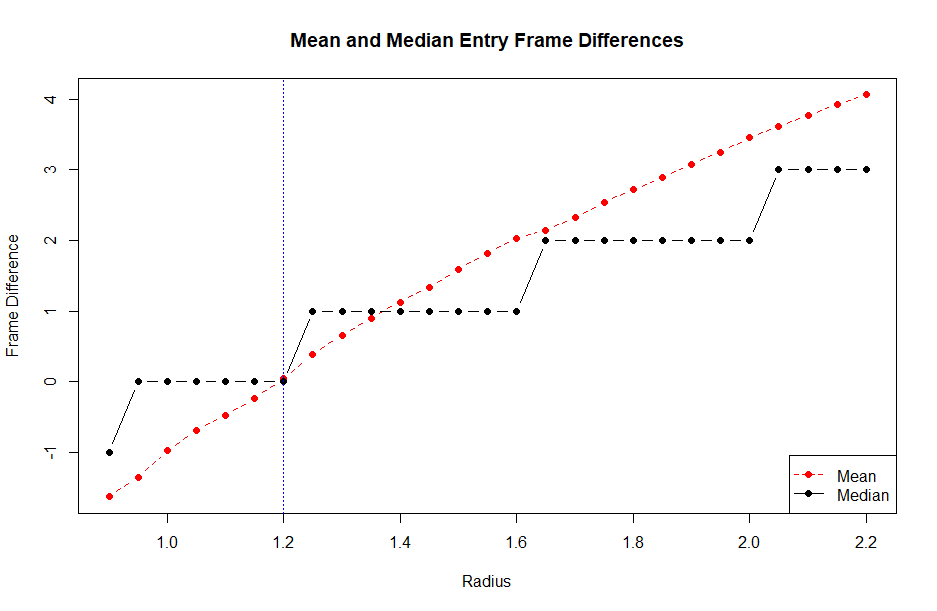
\includegraphics[width=4.6875in,height=\textheight]{Images/entryDiffs.png}

}

\caption{\label{fig-frameDiffs}The mean and median frame differences for
different radii. The dashed blue line at 1.2 signifies the optimal
value.}

\end{figure}%

Figure~\ref{fig-frameDiffs} shows the values for meanEntryDiff and
medianEntryDiff for different zone sizes. The optimal radius appears to
be 1.2 yards, as both the mean and median are centered at 0. This means
that on average, when defenders of interest have a zone with a radius of
1.2 yards around them, the first time the ball-carrier enters a zone is
the same as the event ``first\_contact'' is recorded, which we are
assuming is the true moment of first contact. If 1.2 yards ends up being
too small of a radius, 1.35 and 1.65 yard radii seem like decent choices
too as they look to have close to symmetric frame differences and are
off by about 1 to 2 frames respectively on average (meaning the
ball-carrier is entering the zone \emph{before} first\_contact).

\begin{figure}

\centering{

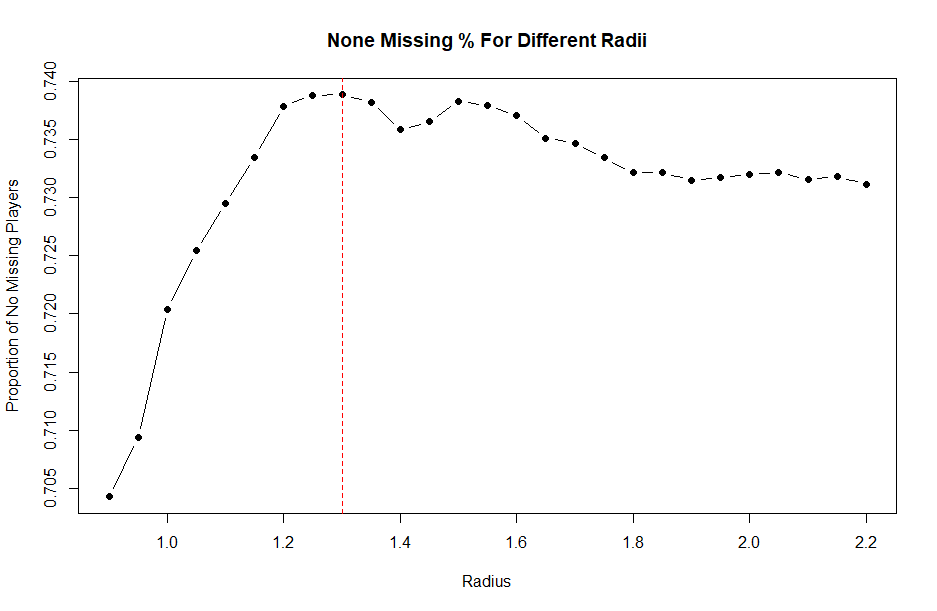
\includegraphics[width=4.6875in,height=\textheight]{Images/noneMissingPct.png}

}

\caption{\label{fig-noneMissingPct}The proportion of plays where no
officially credited tacklers are missed in our predicted tackler list.
The red dashed line indicates the radius with the maximum proportion.}

\end{figure}%

Figure~\ref{fig-noneMissingPct} tells us the proportion of plays where
we correctly identify every officially credited tackler. We see that
1.25 and 1.3 yards are both very similar and have the largest
proportions, meaning that zones with those radii miss the least amount
of official tacklers. This is very similar to the optimal value of 1.2
yards from Figure~\ref{fig-frameDiffs}, and we can see that 1.2 also has
one of the largest proportions here. These results along with the
previous ones indicate that the optimal radius is likely around the 1.2
to 1.3 yard range.

We will not be showing plots for correctPct or extraPct here as their
results were not useful and had little value for interpretation. They
both exhibited highly linear trends, with correctPct decreasing and
extraPct increasing as radius increases. This makes sense from a logical
standpoint--most plays only have one or two tacklers involved in the
actual tackle, and the larger the zone size, the more zones the
ball-carrier will enter in a play. Thus, correctPct will decrease as for
large zones we are often adding far more players than are typically
credited, and extraPct will of course increase for the same reason.

Of all the proposed metrics, we have the most faith in the mean/median
frame differences as they are the stats most directly related to the
actual moment of contact. There may be issues with the
``first\_contact'' event, but it is the closest thing we have in the
data to a definitive moment of contact, so a stat that is directly
involved with ``first\_contact'' seems more reliable for estimating a
contact zone. With this in mind, we believe that 1.2 is the optimal
radius for a contact zone for defensive backs and linebackers.

\subsection{Visual Inspection of Zone
Sizes}\label{visual-inspection-of-zone-sizes}

After evaluating a zone size numerically, we wrote a function called
\texttt{plotGames()} that allows the user to visualize an animation of
any play in our filtered data with contact zones of radius \(r\). To
evaluate our zones, we would look at the animation and then compare to
replays of the real plays to see if our zones seemed to accurately
reflect the play. PDFs cannot support the playback of .gif or .mp4
files, so Figure~\ref{fig-animated} shows several frames from one of the
sampled games.

\begin{figure}

\centering{

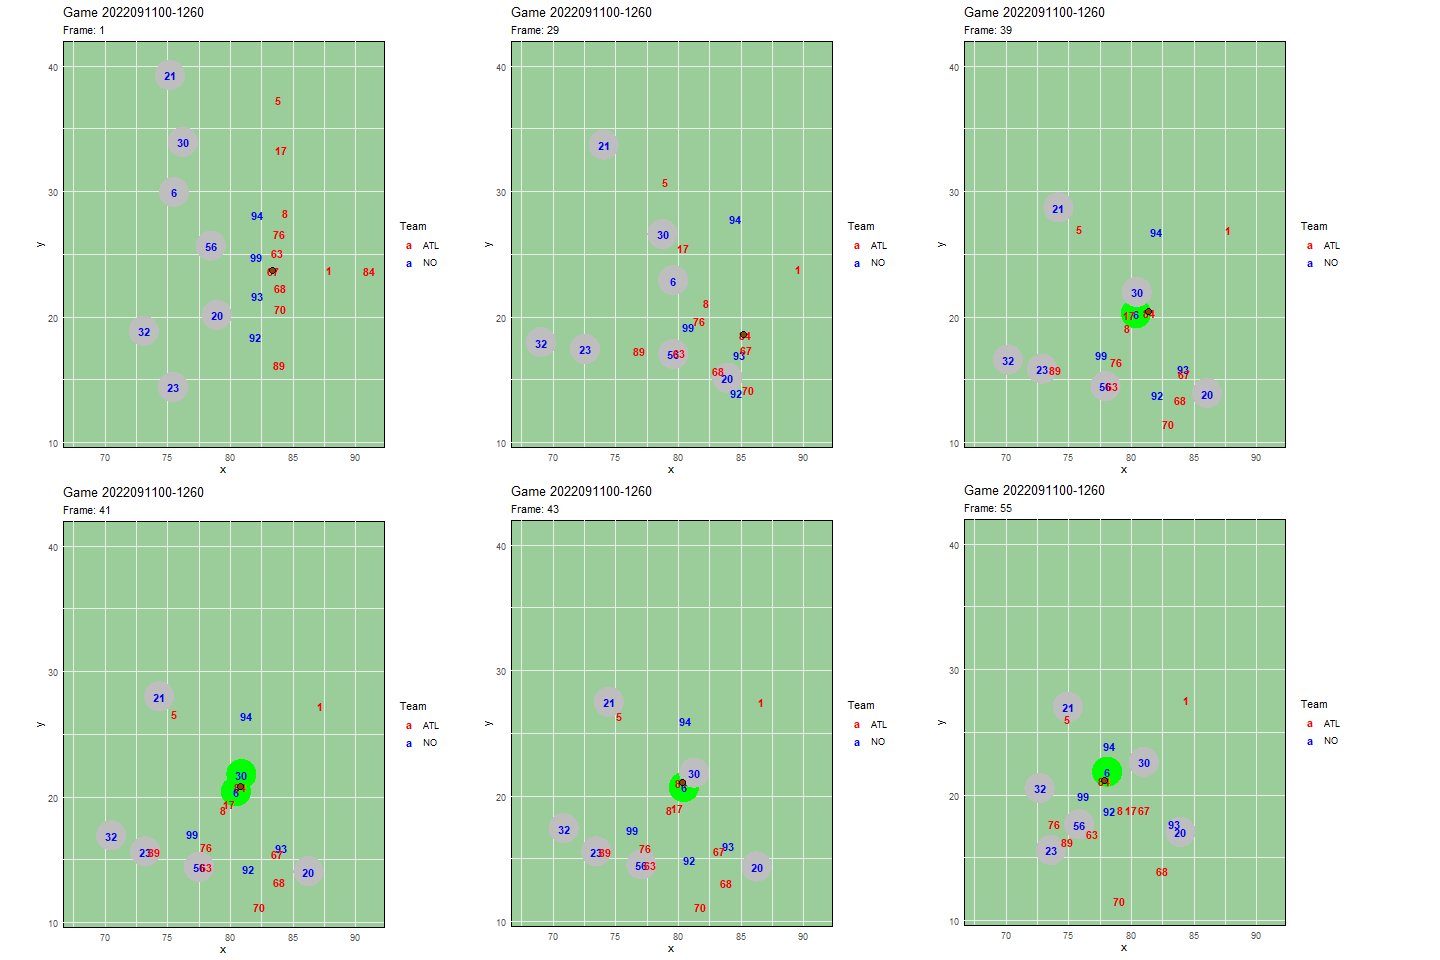
\includegraphics{Images/playFrames.png}

}

\caption{\label{fig-animated}Six frames from a play in the ATL vs NO
Week 1 game in 2022. Top-right image is first contact, where the
ball-carrier (number 84) first comes into contact with a DOI (number 6).
Bottom-left shows another DOI (number 30) who comes in and briefly makes
contact. The play ends on frame 55 in the bottom-right with 6 finishing
the tackle.}

\end{figure}%

If you compare this game to the
\href{https://nfl-video.com/new-orleans-saints-vs-atlanta-falcons-full-game-replay-2022-nfl-week-1}{real
game footage} (the play in question starts at 41:52), you can see that
the zones seem to coincide well with the plays. Player 6 and player 30
both make contact at almost the same point. 30 dives at the ball-carrier
and hits them before falling to the side. 6 wraps around the
ball-carrier and ends up actually bringing them down. This is reflected
very accurately in our data, as 30 only comes into contact for a couple
frames (when he dives), but 6 stays with him all the way through first
contact. If the circle was smaller, it is possible the ball-carrier
would never have entered 30's zone, and if it was bigger then they may
have stayed in 30's zone as even though 30 fell to the side, they still
are relatively close the ball-carrier.

This is just one play of many, but across the games we watched for the
most part a zone with a radius of 1.2 yards seems approximately accurate
to what happens in a real play. It's not perfect of course, but it does
seem to be a good estimate.

\section{Discussion}\label{discussion}

The main goal of this project was to make future work easier for any
researchers interested in analyzing tackling data. Currently, there are
significant issues with identifying when a tackle begins in the tracking
data, as the ``first\_contact'' event has issues such as not being able
to account for multiple tacklers on a play. With our recommendation of a
zone that is centered around each defensive back and linebacker with a
radius of 1.2 yards, we provide an alternative way to measure the
beginning and end of a tackle that is able to handle multiple tacklers
on a play.

Future research that could benefit from incorporating these contact
zones include any tackling analysis that revolves around analyzing
multiple defenders within a play. For instance, one could take the idea
of dividing credit among offensive players for a play from
\citet{Yurko2019} and apply that to defenders. Credit could be assigned
through metrics such as who had the ball-carrier in their zone the
longest or who caused the biggest shift in velocity of the ball-carrier.
We leave the rest of the details to future researchers who may be
interested.

Other research that could benefit from the zones are analyses around
individual tackles, specifically about what happens across the timespan
of a tackle. We could foresee potential metrics that may be able to be
derived from this sort of analysis, such as which defenders can minimize
expected yards after contact or create the largest shifts in momentum of
the ball-carrier (i.e.~who can consistently bring down a ball-carrier
the fastest?).

The data the NFL provides for the competition comes with a variable
called pff\_missedTackles, that is a dummy variable that indicates if a
player missed a tackle on a play. The data is created by Pro Football
Focus, an organization that does a lot of work with American football
statistics. The zones in this paper could provide an alternative way to
assess missed tackles judging by when a ball-carrier enters and leaves a
zone without being tackled. This could also be reframed as missed tackle
opportunities, where we can analyze situations where the ball-carrier
was in a player's zone but they did not make contact. We could see which
players capitalize the most on having a ball-carrier in their zone
versus those who cannot seem to make contact or finish a tackle.

\subsection{Future Work Involving contact
zones}\label{future-work-involving-contact-zones}

There is still much work to be done concerning the analysis in this
paper as well. Our chief concern is the lack of contact zones for
defensive linemen. One could just assign them a zone of radius 1.2 yards
like the other defenders, but we think more research needs to be done to
incorporate blockers before adding zones for linemen. It's also possible
that linemen need to be analyzed separately, as the zone that best fits
defenders who are primarily pass defense may not work best for those who
are mainly focused on stopping runs and sacking quarterbacks. In fact,
it may be worth looking into separating defensive backs and linebackers
and estimating separate zones, or potentially going even further and
creating dynamic zones for each individual player. This would require a
lot more effort, but at the moment we are assuming everybody has the
same ``reach'' but that may not be an accurate reflection of reality.

Something else that is not an accurate reflection of reality is an
assumption we have been holding throughout this entire paper: that the
contact zone is a circle. This is actually not physically possible in
real life, as a defender cannot tackle somebody who is behind them.
Realistically, the zone should be a semi-circle or a cone directly in
front of the defender, which should not be too difficult to create given
that the tracking data includes the orientation of the players. While a
circle is not a good approximation of a real contact zone, we do not
believe it ruins this analysis or causes much error as throughout a
play, it is very rare for a defender to ever have their back to an
active ball-carrier, especially if they are close enough to each other
that we would consider them to potentially be in contact with each
other. Still, updating the zone to a more realistic shape will most
likely offer some improvements to the analysis, if not just making it
more reflective of the real world.


\renewcommand\refname{References}
  \bibliography{references.bib}


\end{document}
